%%
%% PumpTransporter.tex
%% Login : <hoang-trong@hoang-trong-laptop>
%% Started on  Mon Nov  2 02:22:59 2009 Hoang-Trong Minh Tuan
%% $Id$
%% 
%% Copyright (C) 2009 Hoang-Trong Minh Tuan
%% This program is free software; you can redistribute it and/or modify
%% it under the terms of the GNU General Public License as published by
%% the Free Software Foundation; either version 2 of the License, or
%% (at your option) any later version.
%% 
%% This program is distributed in the hope that it will be useful,
%% but WITHOUT ANY WARRANTY; without even the implied warranty of
%% MERCHANTABILITY or FITNESS FOR A PARTICULAR PURPOSE.  See the
%% GNU General Public License for more details.
%% 
%% You should have received a copy of the GNU General Public License
%% along with this program; if not, write to the Free Software
%% Foundation, Inc., 59 Temple Place, Suite 330, Boston, MA 02111-1307 USA
%%

\chapter{Pumps and Exchangers}
\label{chap:models-pumps}
\label{chap:exchangers}
\label{chap:pumps}


\section{Introduction}
\label{sec:introduction-15}

The cell membrane is permeant to water and small ions (e.g. $\Na$), but
impermeant to many cation/anion ionic ions \citep{overbeek1956}. 

The distribution of diffusible ions across the semi-permeable membrane is given
in Donnan equilibrium. Water diffuses into the cell via passive diffusion
(osmosis) or through specialized channels called {\bf aquaporins}. If this
process continue, the cells will inevitably rupture. Even though the plasma
membrane of animal cells are not as tough as cellulose cell wall of plants, it
still possess the remarkable property of maintaining a relatively constant
volume throughout the cell life by the means of excretory system. For example,
to prevent lysis, a red blood cell can diffuse an amount of water of about 250
times its volume across the membrane every
second\footnote{\url{http://www.vivo.colostate.edu/hbooks/cmb/cells/pmemb/osmosis.html}}
at a net amount (osmosis) is equally zero.

\begin{framed}

  Diffusion of water across the membrane from area of high concentration to area
  of low concentration- osmosis - generate a pressure called {\bf osmotic
  pressure}. The pressure inside the cell against the osmotic pressure is called
  {\bf hydrostatic (``water-stopping'') pressure} since when the two pressures
  are equal, the movement of water will stop.
\end{framed}

How about cations like $\Na$ or $\Ca$? To avoid cell swelling due to $\Na$ leak
into the cell, $\Na$ are extruded through an active transport mechanism (i.e.
using energy) - Sect.\ref{sec:ATPase}. The active transport mechanism using
energy for volume maintenance has been proposed since
1960s~\citep{Leaf1959,Tosteson1960}.  Such carrier-like mechanism is carried out
by the so-called exchangers and/or pumps in which the transporatation of an ion,
typically, is coupled with the movement of another ion, in the inverse direction
and/or consumption of some energy molecules. Pump-leak hypothesis is the widely
accepted mechanism for cellular modelling.

Except for the $\NaCa$ exchanger, the other process are active,
i.e. require energy, ATP. Thus these pumps are known as ATP-driven
pumps.  As the activation of these exchangers are ATP-dependent, a
thermodynamics and energetic model for the exchangers is important, as
it can help simulate the cells at conditions where the cell metabolism
is compromised. The details model of these active transports will be discussed
in the next chapters. In this chapter, we will describe the difference and
similarity in structure, functions and mechanisms of these active transports.


\section{1. $\Ca$-ATPase}
\label{sec:Ca-ATPase}

The class formed by $\Ca$-ATPase pumps is designated as types IIa and IIb of
P-type ATPase (or P$_2$) subfamilies - Sect.\ref{sec:P-ATPase-classification}
\citep{Vangheluwe2009, Brini2009}.

$\Ca$-ATPase pump:

\begin{itemize}
  \item Plasma Membrane $\Ca$-ATPase (PMCA) pump: extrude  $\Ca$
    out of the cell via sacrolemma (Sect.\ref{sec:PMCA} - Chap.\ref{chap:PMCA}). 

  \item Sarco(endo)plasmic Reticulum $\Ca$-ATPase (SERCA) pump: resequestering
$\Ca$ back to SR/ER 
(Sect.\ref{sec:SERCA_pump} - Chap.\ref{chap:serca-pumps-models}).

  \item SPCA (secretory-pathway $\Ca$-ATPases)
\end{itemize}

SPCA is mainly found in the membrane of Golgi apparatus, responsible for
transporting $\Ca$ ions, and \ce{Mn^2+} (of high affinity), from the cytosol to
the lumen of the Golgi.  Due to sequence similarity, SERCA and SPCA are
classified as $P_{2A}$ branch; while PMCA belongs to $P_{2B}$ branch. SERCA  has
2 $\Ca$-transport sites; while SPCA has only one.

\subsection{distribution}
\label{sec:Ca-ATPase-distribution}

See Sect.\ref{sec:P-ATPase-distribution}, and
\begin{itemize}
  \item PMCA - Sect.\ref{sec:PMCA-distribution}
%  \item NCX - Sect.\ref{sec:NCX-distribution}
%  \item NaK - Sect.\ref{sec:NaK-distribution}
  \item SERCA - Sect.\ref{sec:SERCA-distribution}
\end{itemize}

\subsection{activator}
\label{sec:Ca-ATPase-activator}


\section{PMCA protein family and structure}
%\subsection{-- PMCA (Plasma Membrane Calcium-ATPase)}
\label{sec:PMCA}
%\section{PMCA}
\label{sec:pmca}

PMCA is a member of the P class of ion-motive ATPases
\citep{pedersen1987a,pedersen1987b} (Sect.\ref{sec:P-ATPase}).
It was discovered in 1966 by Schatzmann. 
The PMCA pump is a minor component of the total protein of the plasma membrane
(less than 0.1\% of total membrane proteins).
An exception is the brain where this value is up to 10 times higher than in
non-excitable cells (Guerini, 1998).

Quantitatively, PMCA is overshadowed by the more powerful NCX in most excitable
tissue like heart; however, even cells in which the NCX predominates, the PMCA
pump is likely to be the fine tuner of cytosolic $\Ca$, as it can operate in a
concentration range in which the low affinity NCX is relatively very
inefficient. Also, it has low transport capacity, at 30Hz (i.e. one PMCA
extrudes 30 ions/sec).

\subsection{ATP, proton (H+) uptake}

PMCA utilizes 1ATP in exchange for 1 $\Ca$ ion out, with some protons uptake
(\ce{H+}). \citep{niggli1982, smallwood1983} showed that the extrusion of 1
$\Ca$ ion consume one ATP molecule, and coupled to $\H$ uptake. Im some cell
types, the coupling ratio  $\ce{Ca^2+}:\ce{H^+}$ is external pH dependent. 
\begin{itemize}
  \item red blood cell: ratio is 1:2 (neutral) at pH = 6.5; and ratio 1:0 at pH
  = 8.5
  \item barnacle muscle cell: ratio is 1:3 at pH = 6.5; and ratio 1:1 at pH=8.2
  
  \item In snail neuron, \citep{thomas2009} showed that PMCA is electroneutral
  with 1$\Ca$:2$\H$, and much less sensitive to pH.
\end{itemize}


\subsection{pumping activity}

Each PMCA molecule pumps 30-100 $\Ca$ ions per second (low capacitiy) yet with
high affinity to calcium (Km = 0.2 $\muM$). As the process of pumping one
calcium ions goes through a number of chemical reaction (Sect.\ref{sec:}), in
other words, the pumping cycling is said to be 30-100Hz.

In T cells, Bautista et al (2002) showed that this pump is the primary means of
$\Ca$ extrusion in T cells and its activity is modulated by $\Ca$-enabling the
cell to adapt to higher $\Ca$ values during T cell activation.  Additionally
once $[\Ca]_i$ returned to baseline levels the PMCA recovered slowly with a time
constant of $\approx$ 4 min providing a 'memory' of previous $[\Ca]_i$.

Its computational model is discussed in Chap.\ref{chap:PMCA}.

\subsection{isoforms}
\label{sec:PMCA-isoforms}

Plasma membrane $\Ca$-ATPase (type IIB).
PMCA is the product of a multigenes family (ATP2B1-4). So, there are
about 30 different isoforms~\citep{Brini2009}. They differs in tissue
distribution, and calmodulin affinity. 

However, there are 4 main isoforms (PMCA1-PMCA4), each is expressed by a
different gene found in rats and humans (Sect.\ref{sec:PMCA-distribution}). As
the four isogenes undergo several types of alternative splicing producing more
isoforms proteins, they create the diversity in PMCA families
\citep{strehler2001}.
  

\textcolor{red}{splicing}: The splicing occurs at two spots defined as A and C,
and leads to the inclusion of one or more exon.  All genes of PMCA families,
except PMCA1, undergo splicing at site A. Splicing on PMCA2 include three exons
(33, 60 and 42 bp). PMCA3 and PMCA4 have no exon inclusion at site A.
Alternative splicing at site C is more complicated.
Example of early notation:
\begin{enumerate}
  \item PMCA2f (no spliced exon), 
  
  \item PMCA2h (inclusion of 42bp exon), 
  
  \item PMCA2g (inclusion of 3 exons of different lengths: 42, 60, 33bp). At
  site C, the isoform with a full 154 bp exon was labeled 'a' and isoform without inserts was labeled 'b'.
  
  \item hPMCA2b and hPMCA4b: with 'h' = 'human' 
\end{enumerate}
To resolve the naming convention, \citep{carafoli1994} suggested using I (no
insertion), II (full exon insertion), and III, IV, etc. (combination of
insertions).  So, PMCA1Cb means PMCA1 (isogene 1), C (splice site C), b (no
insert). 


\textcolor{red}{Length}: The four main isoforms of PMCA has length  $\sim 1200$
amino acids, with 10 transmembrane helices M1-M10, essentially same membrane
topology properties of SERCA (Sect.\ref{sec:SERCA_conformations}).
Crystallization of PMCA is particularly challenging because there is no natural
source from which this protein can be obtained in large quantities.

Before the evailability of PMCA's 3D structure ~\citep{carafoli1994}, molecular
modeling work of PMCA based on structure of SERCA
(Sect.~\ref{sec:introduction-13}) has shown similar general structures, with 3
main A-, N- and P- domains. The long COOH-terminal contains most of the
regulatory domains (Sect.\ref{sec:PMCA-activator}, Sect.\ref{sec:PMCA-inhibitors}).

\subsection{distribution}
\label{sec:PMCA-distribution}

The PMCA was first discovered in erythrocytes (Schatzmann 1966) and was
recognized as a transmembrane protein to pump $\Ca$ out \citep{schatzmann1966}.
It was purified in 1979 using a calmodulin affinity column (Niggli et al. 1979),
and cloned about 10 years later (Shull and Greeb 1988; Verma et al. 1988).

It was then described and characterized in numerous other cell types
(review:\citep{carafoli1991,carafoli1994,carafoli2000}). 

PMCA2 and PMCA3 activate more rapidly and thus are found in excitable cells
(nerons and muscle tissues).

See Sect.\ref{sec:Ca-ATPase-distribution}.


\subsection{disease}

Genetic defects of PMCA function produce disease phenotypes: 

{\bf deaf}: the best characterized is a form of deafness in mice and in humans
linked to PMCA2 mutations. 

{\bf ataxia}: A cerebellar X-linked human ataxia has recently been found to be
caused by a mutation in the calmodulin-binding domain of PMCA.

%\subsection{3D structure}
\subsection{regulators}

As a P-type ATPase (sect.\ref{sec:P-ATPase}, PMCA has 2 main conformations: E1
and E2. 
\begin{itemize}
  \item The conformation E1 (with bound ATP) has high cytosolic $\Ca$-binding
affinity.

  \item The intermediate conformations E1P and E2P are phosphorylated forms,
  i.e.  E1 with catalic aspartic acid domain phosphorylated by ATP. 
  
  \item The conformation change from intermediate form E1P to E2P brings $\Ca$
  to the extracellular side, and promotes $\Ca$ release before the cleavage of
  the phosphorylated intermediate.
  The cleavage brings the pump to E1 conformation.

  \item E2 (without ATP) is with low $\Ca$ affinity (which enables bound $\Ca$
  to be released on the extracellular side), Fig.\ref{fig:pmca_E1E2}.

\end{itemize}


\begin{figure}[hbt]
  \centerline{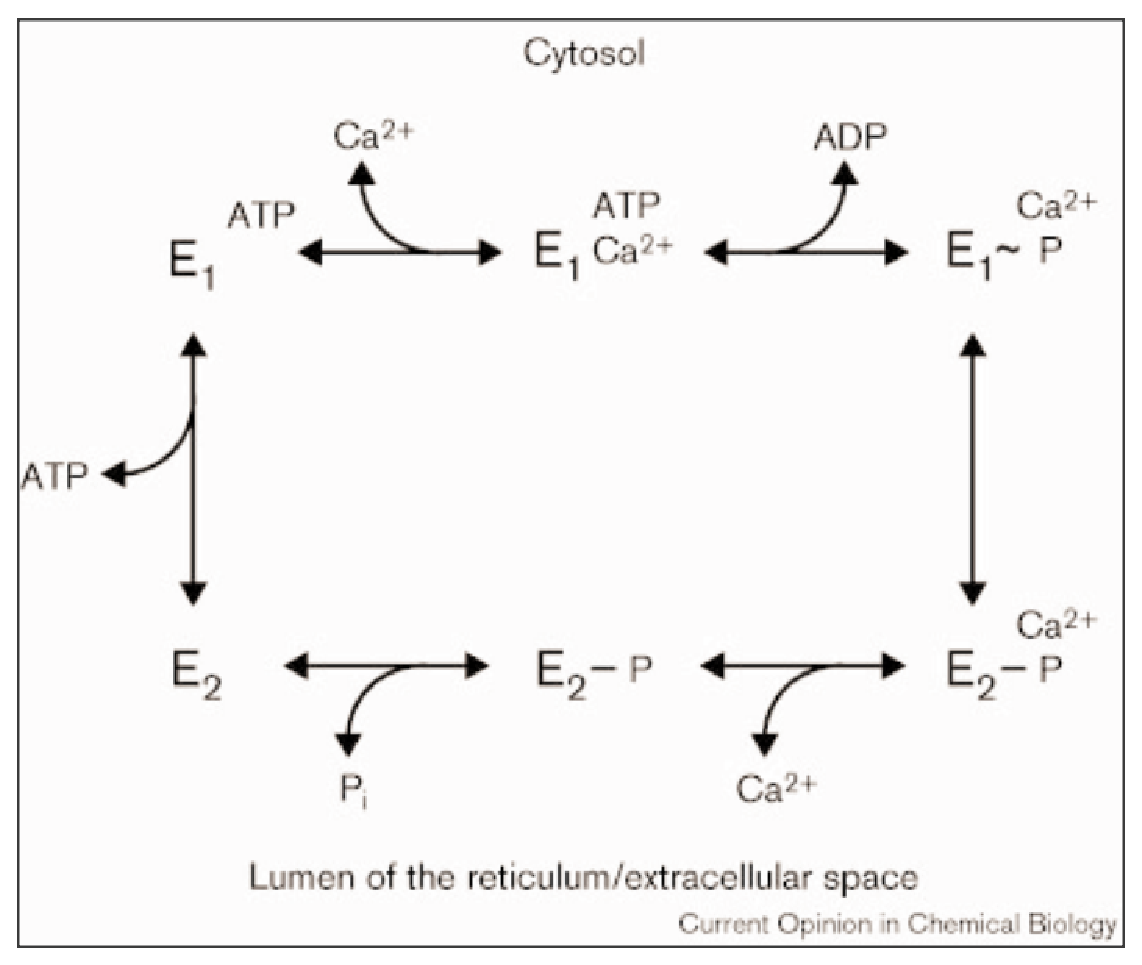
\includegraphics[height=5cm,
    angle=0]{./images/pmca_E1E2.eps}}
\caption{A simplified reaction scheme of PMCA \citep{carafoli2000}}
\label{fig:pmca_E1E2}
\end{figure}

% 
% \begin{itemize}
%    
%    \item calmodulin binding domain
% 
%    \item $\ca$ binding motifs at upstream or downstream of calmodulin binding domain. 
% \end{itemize}
% 
% \begin{framed}
%   PMCA only pumps $\ca$ efficiently when activated by calmodulin. 
%   Role of NCX and PMCA in other cells:
% 
% \begin{enumerate}
%   \item beta cells: \citep{herchuelz2007}
% \end{enumerate}
%   
% \end{framed}
% 

\subsection{-- activators}
\label{sec:PMCA-activator}

PMCA is regulated by different factors: Calmodulin, protein kinases, acidic
phospholipids, oligomerization, proteases, and G proteins \citep{monteith1995}.
\citep{gao2004} studied PMCA3 on crayfish antennal gland showed an upregulation
during the period of $\Ca$ transient. 


\textcolor{red}{\bf ATP}: ATP is critical for PMCA's operation.
PMCA is powered by the hydrolysis of ATP, i.e. with 1ATP for extrusion 1 $\Ca$
ion. Under normal condition, if we assume ATP production is enough, we can model
without taking into account the level of ATP. One way to take into account the
effect of ATP depletion is reducing $v_\max$ (the maximal transfer rate) or
$\bar{I_\pmca}$.

\textcolor{red}{Calmodulin} (Sect.\ref{sec:calmodulin}): CaM interacts with high
affinity to the cytosolic C-terminal tail of PMCA.  A second calmodulin-binding
domain with lower affinity is present in some splicing variants of the pumps.

The calcium binding site
encompass a calmodulin-binding domain.
Thus, $\Ca$/Calmodulin binding can enhance PMCA activity, by increasing the affinity
of $\Ca$ ions to 20-30-fold higher, i.e. $K_d \sim 0.4-0.5 \muM$, and increasing
the pump rate (possibly 10-fold).

\textcolor{red}{\bf Calcium}: 
The binding to $\Ca$ is very high, i.e. $K_d = 10-20$ ($\muM$) at resting state
and can decreases to $< 1 \muM$ following calmodulin interaction. The removing
rate of $\Ca$ from the intracellular media is low, the cycle is $\sim 30$ Hz for
each molecule (i.e. low capacity). This is in contrast to NCX, which has low
binding affinity but high capacity. So, PMCA work effectively at low $[\Ca]_i$
to extrude $\Ca$, and NCX work effectively to pump $\Ca$ at high $[\Ca]_i$.

\begin{itemize}
  
\item PMCA1 and PMCA4 are ubiquitous, yet with low calmodulin affinity
  (i.e. high dissociation constant $K_d=40-50$ (PMCA1b), $K_d=30-40$ (PMCA4b)

\item PMCA3 restricted to nervous system and PMCA2 is restricted to
  nervous system and mammary gland, with high calmodulin affinity
  ($K_d=2-4$ (PMCA2b), $K_d=8$ (PMCA3b))
\end{itemize}
NOTE: In some pump types, calmodulin could be a permanently bound subunit of the
enzyme, e.g. PMCA2 has abnormally high affinity to calmodulin. In such cases,
we typically ignore the role of [Calmodulin] concentration
(Sect.\ref{sec:calmodulin}).

\textcolor{red}{acidic phospholipids and long-chain polyunsaturated fatty
acids}: In the absence of calmodulin, PMCA is activated (i.e. increase the $\Ca$
affinity and pumping rate) by acidic phospholipids. In vivo, 
where high concentrations of acidic phospholipids is present, it appears
likely that PMCA is in activated state permanently, e.g. about 50\%
of maximal stimulation. 

\textcolor{red}{PKC} (Sect.\ref{sec:PKC}): PKC activates pump;  with PKC in
turns is activated by DAG (Sect.\ref{sec:DAG}).


\begin{mdframed}

In squid giant axons, Na influx can have a magnitude of 30 nmol/(cm$^2$.s), Na
pump (Na/K-ATPase) flux 30 pmol/(cm$^2$.s) and $\Ca$ pump (PMCA) flux 30
fmol/(cm$^2$.s), or the ratio is $10^6:10^3:1$. So, the effect of PMCA on
removing $[\Ca]_i$ is not much. 
\end{mdframed}


\begin{mdframed}
There are two sites (1) binding Calmodulin, (2) binding $\Ca$. 

The binding site involved in $\Ca$ translocation is different between SERCA and
PMCA. In SERCA pump and other P-type, this site is an acidic residue in helix
M5; but not in PMCA \citep{carafoli2000}. The residues know to play a critical
role to $\Ca$ transport is Glu432 (in helix M4), Asp879 and Asp883 (both in
helix M6). The stoichiometry 1$\Ca$:1ATP for PMCA, and 2$\Ca$:1ATP for SERCA
pump.

\end{mdframed}



Two key features of the PMCA are its stimulation by $\Ca$-calmodulin and by
PKC-dependent phosphorylation (Bers, 2001). 
\begin{itemize}
  \item $\Ca$-calmodulin stimulate $v_\max$ by decreases its $\Km(\Ca)$ by one
  order of magnitude, from 10-20$\muM$ to 0.5 $\muM$. Also, the sensitivity to
  $\Ca$-calmodulin varies at different isoforms of PMCA
  (Sect.\ref{sec:PMCA-isoforms})

NOTE: A $\Kd$ of about 1 nM has been measured.

  
  \item 
\end{itemize}

The activity of the pump is insensitive to the membrane potential. 


Historically, \textcolor{red}{Calmodulin is the major activator} to stimulate
the pump, which stimulates $v_\max$ of the pump, and increase $\Ca$ affinity by
decreasing $K_d$(Ca) by one order of magnitude (from 10-20$\muM$ to 0.5$\muM$)
\citep{carafoli1994}. So, the pump is aka plasma-membrane Ca-Calmodulin-ATPase
pump. In the absence of Calmodulin, the next activator is acidic phospholipid
and long-chain polyunsaturated fatty acids \citep{ronner1977}. Acidic
phospholipid binds 2 sites in the pump molecule: one is calmodulin binding
domains, and the other is a stretch of about 40 predominantly amino acids in the
cytosolic loop connecting domains 2 and 3.
\begin{enumerate}
  \item Calmodulin-binding domain is the amphiphilic helix in its \ce{NH2}- and
  COOH-terminal
\end{enumerate}

\subsection{-- inhibition, de-inhibition}
\label{sec:PMCA-inhibitors}
\label{sec:PMCA-deinhibitors}

\textcolor{red}{\bf orthovanadate}:
As a P-type ATPase (Sect.\ref{sec:P-ATPase-inhibitor}), the inhibitors are
orthovanadate and \ce{La^3+}. 

\textcolor{red}{\bf Ca-calmodulin}: The  ATP-binding site of PMCA also bind with
CaM-Ca. So CaM-Ca serves as an inhibitor to PMCA.


\textcolor{red}{\bf Phospholamban}: Another inhibitor is phospholamban, yet it
is not found in brain.


The inhibition-deinhibition process is very similar to SERCA pump whose activity
is maintained in a repressed state by accessory protein phospholamban (PLN) -
Sect.\ref{sec:phospholamban}.

The relief of inhibition is brought about by the phosphorylation of phospholamban by
cAMP-dependent and calmodulin-dependent protein kinases. The binding sites for
the two inbitory peptides are very close to the active site in homologous region
of the two pumps, Fig.\ref{fig:SERCA_PMCA}. 

\begin{figure}[hbt]
  \centerline{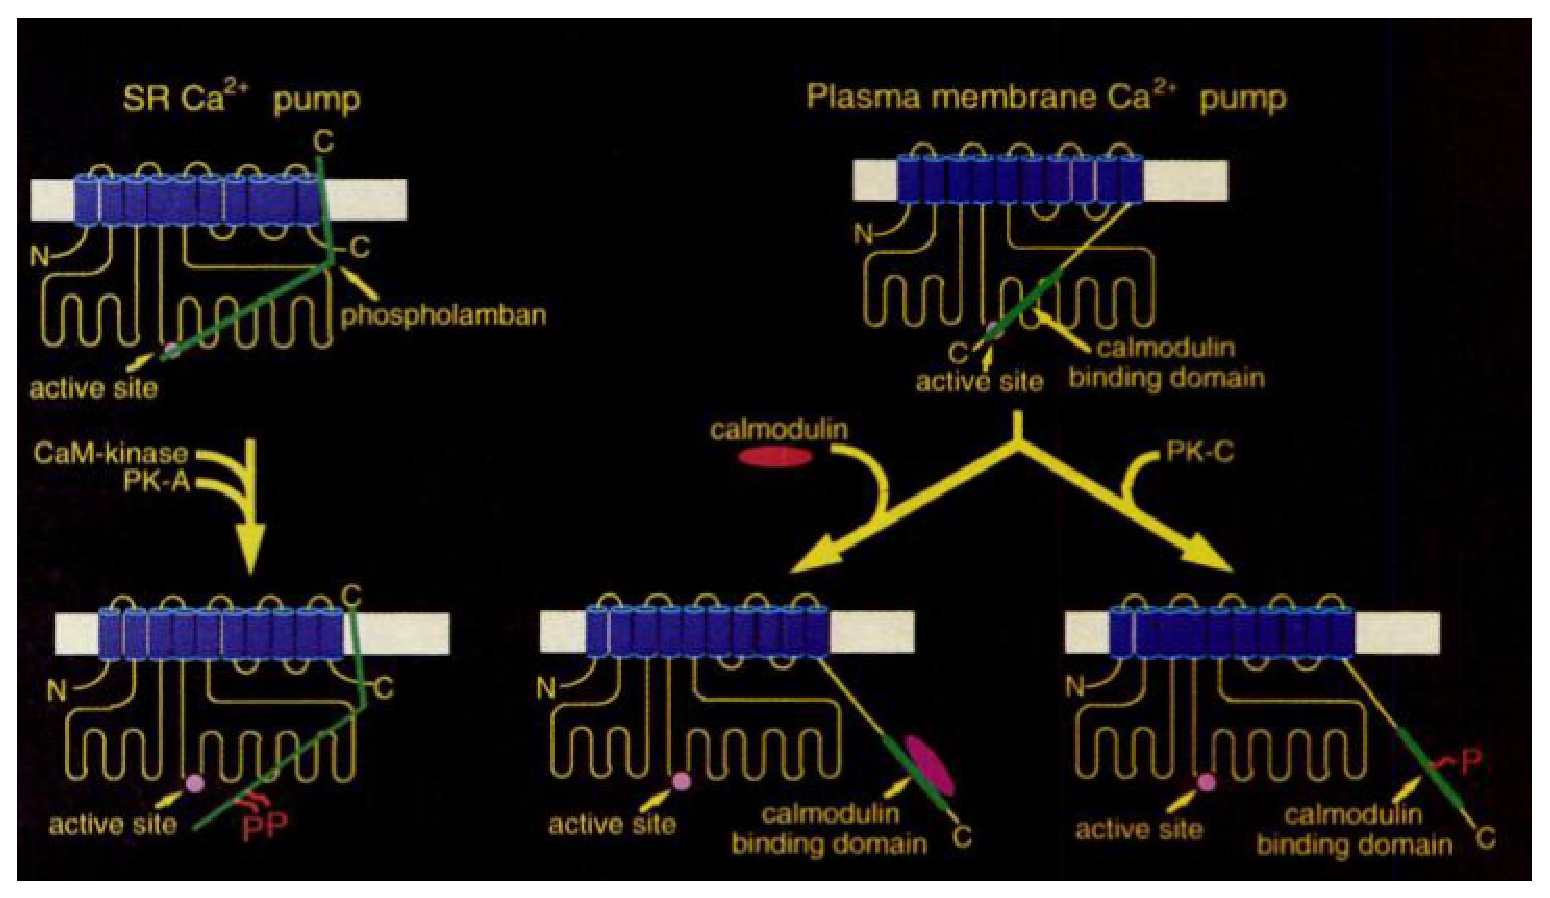
\includegraphics[height=5cm,
    angle=0]{./images/SERCA_PMCA.eps}}
\caption{SERCA is kept at inhibited state by an intrinsic protein PLN, which
can be removed by either CaM-kinase or PKA. PMCA is kept at an inhibited state
by its own COOH-terminal calmodulin-binding domain; which can be activated by
either binding calmodulin or phosphorylation using PKC}
\label{fig:SERCA_PMCA}
\end{figure}



\section{SERCA pump}
\label{sec:SERCA_pump}

SERCA ATPase (type IIA): transport 2 $\Ca$ per turnover with high affinity,
probably exchange 1-2 $\H$. There are 3 main isoforms: SERCA 1, SERCA 2 and
SERCA 3. For modelling SERCA pump, we read Chap.~\ref{chap:serca-pumps-models}.

  
\subsection{isoforms - subfamilies}
\label{sec:SERCA-isoforms}

There are three main isoforms of SERCA (SERCA1-3). SERCA1 gene (ATP2A1) (on
chromosome 16 of human) produces two isoforms of the $\Ca$-ATPase, by
alternative splicing of the primary gene product \citep{MacLennan1985,
brandl1986}, i.e. SERCA1a and SERCA1b. SERCA2 gene (ATP2A2) (on chromosome
12 of human) also produces at least two isoforms (SERCA2a, SERCA2b). SERCA3 gene
(ATP2A3) produces more isoforms (SERCA3a-f).

In human, 3 genes (ATP2A1-3) generates multiple SERCA isoforms (SERCA1a,b,
SERCA2a-c, SERCA3a-f)

Nowadays, we know that SERCA pump can function as a monomer
\citep{carafoli2000}. So, oligomerization is not important for SERCA's normal
function. The expression level of SERCA pumps and their role in the uptake of
$\Ca$ from the myoplasm is species specific \citep{periasamy2001}. 


%\subsection{3D structures}

The molecular mass of all SERCA types are about 110kDa. The 3D structure of
SERCA pump from electron microscopy (14$\AA$) first discovered in 1986
\citep{taylor1986}, and then at a higher resolutions (8$\AA$) in a few years
later \citep{toyoshima1993,zhang1998}. 
% The 2.6$\AA$ resolution by X-ray
% crystallography was done in 2000 by \citep{toyoshima2000}.
SERCA1 is abundant in skeletal muscle and was the first to have crystalized
structure, i.e. $\Ca$-ATPase in $\ce{E2\cdot Ca2}$
conformation~\citep{toyoshima2000} (at 2.6$\AA$).
\textcolor{red}{This will provide insights into the mechanism of
  catalytic pump cycle}~\citep{stolkes2003}.
  
Mutagenesis allows identifying the important residues that controls the $\Ca$
transport pathway. A SERCA molecule has a domain of 10 transmembane (TMs)
$\alpha$-helices (M1-M10), a stalk sector made up of helical extensions of
transmembrane helices, and a cytoplasmic $\beta$-strand. The phosphorylation and
nucleotide binding domains attached to the stalk domain at a distance of 60$\AA$
from the transmembrane domain.

The N-terminal sequences are similar: Met-Glu-X(Ala, Asn, Glu, Asp)-X(Ala, Gly,
Ile). The C-terminal are different
\begin{enumerate}
  \item The C-terminus of SERCA1a has \citep{martonosi2003} 
  \begin{enumerate}
    \item Glycine residue at C-terminus in rabbit
    \item Alanine residue at C-terminus in chicken
    \item C-terminus in lobster is blocked
  \end{enumerate}
  Glycine at the C-terminus is replaced by sequence
  Asp-Pro-Glu-Asp-Glu-Arg-Ag-Lys to become SERCA1b. 
  
  \item The C-terminus of SERCA2 is Pro-Ala-Ile-Leu-Glu. SERCA2b is
  characterized by a long C-terminal extension of 50 amino acids residues ending
  in Trp-Ser. 
  \item The C-terminus of SERCA3 is Asp-Gly-Lys-Lys-Asp-Leu-Lys.
\end{enumerate}

The transmembrane domains are almost entirely $\alpha$-helical with short loops
on the lumenal and cytoplasmic surface.
\begin{itemize}
\item 2 large cytoplasmic loops between transmembrane helices M2/M3
  and M4/M5 form 3 cytoplasmic domains. One of them forms the
  phosphorylation (P) site (on top of M4/M5), and nucleotide binding
  (N) domain.

\item third cytoplasmic loop, dubbed the transduction or actuator (A)
  domain
\end{itemize}

PMCA has 5 units protruding into the cytosolic side, yet SERCA has only 3
\begin{enumerate}
  \item amino-terminal unit: no important functional domain
  \item second unit: lack the acidic phospholipid binding site, so SERCA is not
  sensitive to acidic phospholipid
  \item third unit: contain the active site
\end{enumerate}

\subsection{distribution}
\label{sec:SERCA-distribution}

\begin{framed}
  \begin{itemize}
  \item SERCA1 is highly expressed in fast-twitch skeletal muscle, and some in
  brown adipose tissue (BAT).
  \item SERCA2 is found on slow-twitch skeletal and cardiac muscle. It has 2
  varianes:  SERCA2a (muscle-specific variant, i.e. excitation-contraction)
  and SERCA2b (housekeeping variant, i.e. maintain basic cellular
    functions).     
  \item SERCA3 differs from the two above isoforms. It has remarkably
    low affinity for cytosolic $\Ca$ (supra $\mu$M), and luminal $\Ca$
    (lower mM). They are found in non-muscular tissues (e.g. blood platelets)
  \end{itemize}
\end{framed}

\subsection{-- neuron}


\subsection{-- heart}


SERCA2a plays an important role in cardiac excitation-contraction
process~\citep{Vangheluwe2006,Periasamy2008}. In addition, in native cardiac SR
environment, SERCA2a is regulated by {\it phospholamban} (PLN or
PLB)~\citep{MacLennan2003} (Sect.\ref{sec:PLN_SERCA}). However, SERCA2b has
higher $\Ca$-affinity than SERCA2a. This higher affinity can be offset by PLN,
which plays a protective role.

SERCA pump also interact reversibly with phospholamban (PLN). There are
evidences of higher concentration of SERCA pumps near the Z-lines and decreases
exponentially toward M-lines \citep{smith1998}.

\subsection{disease}

Deffects on SERCA1, but not SERCA2, can cause some forms of Brody's disease
\citep{MacLennan2000}. This suggests SERCA1 and SERCA2 are independently
regulated.


\subsection{regulators}

6 residues in TMS4, TMS5, and TMS6 are found to be critical to high
$\Ca$-binding and translocation. 

The residue in TMS8 is found to be important to high $\Ca$-binding only. Also,
the sequences connecting between TMS4 and TMS5 play a role in forming the
phosphorylated intermediate state (E1P or E2P states), suggesting their
involvement in the binding of ATP \citep{carafoli2000}. Another highly conserved
region in $\beta$-strand portion of the first cytoplasmic loop control the
transport of $\Ca$, not in forming the phosphorylated intermediate.



\section{2. Na/K pump}
\label{sec:NaK_pump}

$\NaK$ ATPase is Type IIc P-type ATPase (Sect.\ref{sec:P-ATPase}).

Na/K-ATPase (type IIC) (abbreviations: NKA) extrudes leaking (in) $\Na$
\citep{skou1957}: for each ATP hydrolyzed (i.e. per turnover) it pumps 3 $\Na$
out and 2 $\K$ in (Chap.\ref{chap:NaK_pump}), Fig.\ref{fig:P-ATPase_type2}.
\textcolor{red}{It helps in maintaining the resting membrane potential}
(Sect.\ref{sec:resting-membrane-potential-range}).

  
% \begin{framed}
% \end{framed}

Na/K-ATPase is a key enzyme to the homeostasis of osmotic pressure, cell volume
and the maintenance of electrochemical gradients across the sarcolemma. Na/K
pump was first identified by~\citep{skou1957} in leg nerves of crab (sciatic
nerve), which brought him the Nobel prize about 40 years later. However, much of
the earlier works on Na/K-ATPase pump used resealed ghost of erythrocyte as the model
system~\citep{post1957, post1960}. Na/K pump nowadays is a member of the P-type
active transporters (Sect.\ref{sec:P-type_ATPase}).
It pumps 3$\Na$ out and 2$\K$ in, for each ATP hydrolysed \citep{post1957}.

More than 1/3 of the ATP consumed by a resting animal is used by
Na/K-ATPase.  Na/K pump can exist in 2 major conformational states:
(1) preferentially bind $\Na$ and ATP, (2) higher affinity for $\K$
and inorganic phosphate Pi. ATP binding facilitates the switching between
the two states (Sect.~\ref{sec:nak-pump:-post}).

\subsection{isoforms}
\label{sec:NaK-isoforms}

$\NaK$-ATPase is the binary complex of an $\alpha$-subunit (4 isoforms:
$\alpha1-\alpha4$), a $\beta$-subunit (3 isoforms: $\beta1-\beta3$) and possibly
a smallest one $\gamma$ subunit \citep{morth2011}. $\alpha$ subunits, which
holds mosts of its functions, belongs to the P-type subfamily IIC \citep{saez2009}.

There are 3 isoforms ($\alpha$-1,-2, and -3) and helps to regulate ion
concentration gradient, i.e. directly affecting resting membrane potential
(Sect.\ref{sec:resting-membrane-potential}).
\begin{enumerate}
  \item $\alpha1$ is the predominant and ubiquitously expressed isoforms

  NOTE: $\alpha-1$ present in kidney and epithelia;

  \item $\alpha2$ is mainly expressed in skeletal, heart, smooth muscle, brain,
  lung and adipose tissue

  NOTE: $\alpha-2$ presents in adult  muscle, heart, neurons, adipocytes and is
  important for $\K$ homeostasis;  

  \item $\alpha3$ is primarily expressed by neurons and heart cells.
 
  NOTE: $\alpha-3$ presents in neuronal cells, smooth muscle, renal collecting
  ducts. This is the drug target, e.g. digitalis glycosides (heart treatment).

  \item $\alpha4$ is only found in testes, and is linked to the mobility of
  spermatozoa.
\end{enumerate}
  
% 29. Peng, L., Martin-Vasallo, P. & Sweadner, K. J. Isoforms of Na,K-ATPase alpha
% and beta subunits in the rat cerebellum and in granule cell cultures.
% J. Neurosci. 17, 3488 - 3502 (1997).
% 30. Pietrini, G., Matteoli, M., Banker, G. & Caplan M. J. Isoforms of the Na,KATPase
% are present in both axons and dendrites of hippocampal neurons in
% culture. Proc. Natl. Acad. Sci. USA 89, 8414 - 8418 (1992).


The $\beta$ subunits is 45kDa proteins that influences $\K$ affinity, and $\H$
pumping efficiency for the case of $\H/\K$-ATPases. In Na/K-ATPase, Tyr
residue is the main interaction point between $\alpha$ and $\beta$ subunits, playing an important
role for E2 stabilizing with bound $\K$. 
\begin{enumerate}
  \item $\beta1$ is found in most tissues, and forms $\alpha1\beta1$ complex
  \item $\beta2$ is predominantly expressed by neurons, and (to some degrees) by
  heart cells in rats
  \item $\beta3$ is found in testes and early development stage of neurons in
  {\it Xenopus laevis}. 
\end{enumerate} 

\subsection{distribution}
\label{sec:NaK-distribution}

\section{3. NCX protein family and structure}
\label{sec:NCX_family}

Sodium-calcium exchanger (NCX) is found after PMCA, yet is the main mechanism of
extruding $\Ca$ out of intracellular media in many cell types. The type of
channels and the relative proportions of NCX and PMCA vary with the cell type,
the NCX being particularly abundant in excitable tissues, e.g., heart and brain.
In $\beta$-cells and the heart, NCX is the predominant mechanism for $\Ca$
extrusion, accounting for 70\% and 90\% $\Ca$ extrusion, respectively.
Modeling NCX is discussed in Chap.\ref{chap:NCX}.

The evidences of coupling between $\Na$ and $\Ca$ was first discovered in late
1960s \citep{reuter1968, baker1969}. Unlike PMCA, NCX requires NO ATP energy,
instead it uses the gradient of $\Na$ between extracellular and intracellular as
the driving force.

\begin{mdframed}

The idea that the source of energy for $\Ca$ extrusion is the inward gradient of
$\Na$ was first demonstrated experimentally in guinea-pig atria
by~\citep{reuter1968}. They first shown the $[\Na]_o$-depenent $\Ca$ efflux and
then, in another paper, shown $[\Na]_i$-dependent $\Ca$ influx, establishing the
concept of bi-directional $\NaCa$ exchanger mechanism\citep{glitsch1970}.

In the absence of external ($\Na$ or $\Ca$) or internal ($\Na$ or $\Ca$),
exchanger cannot mediate a significant net influx or efflux of $\Ca$. So, they
came to a conclusion for the coupled countertransport between $\Na$ and $\Ca$;
rather than both competing for a binding site involved in $\Ca$ transport. 
The protein that does this function is nowadays known as $\NaCa$ exchange (NCX)
which can move $\Ca$ either inward or outward depending on the electrochemical
gradient of $\Na$.
\end{mdframed}

{\it Researchers in NCX are (England: Baker, Blaustein,
Hodgkin.., USA: Martin, DeLuca...)}.


\subsection{isoforms}
\label{sec:NCX-classification}
\label{sec:NCX-isoforms}

There are 5 genes that have been identified in mammals to encode for
exchangers: $\NaCa$ exchanger family (NCX1, NCX2, NCX3), $\K$-dependent $\NaCa$
(NCKX1, NCKX2).

\subsection{-- NCX1-3}
\label{sec:NCX-conformation}

\begin{figure}[hbt]
  \centerline{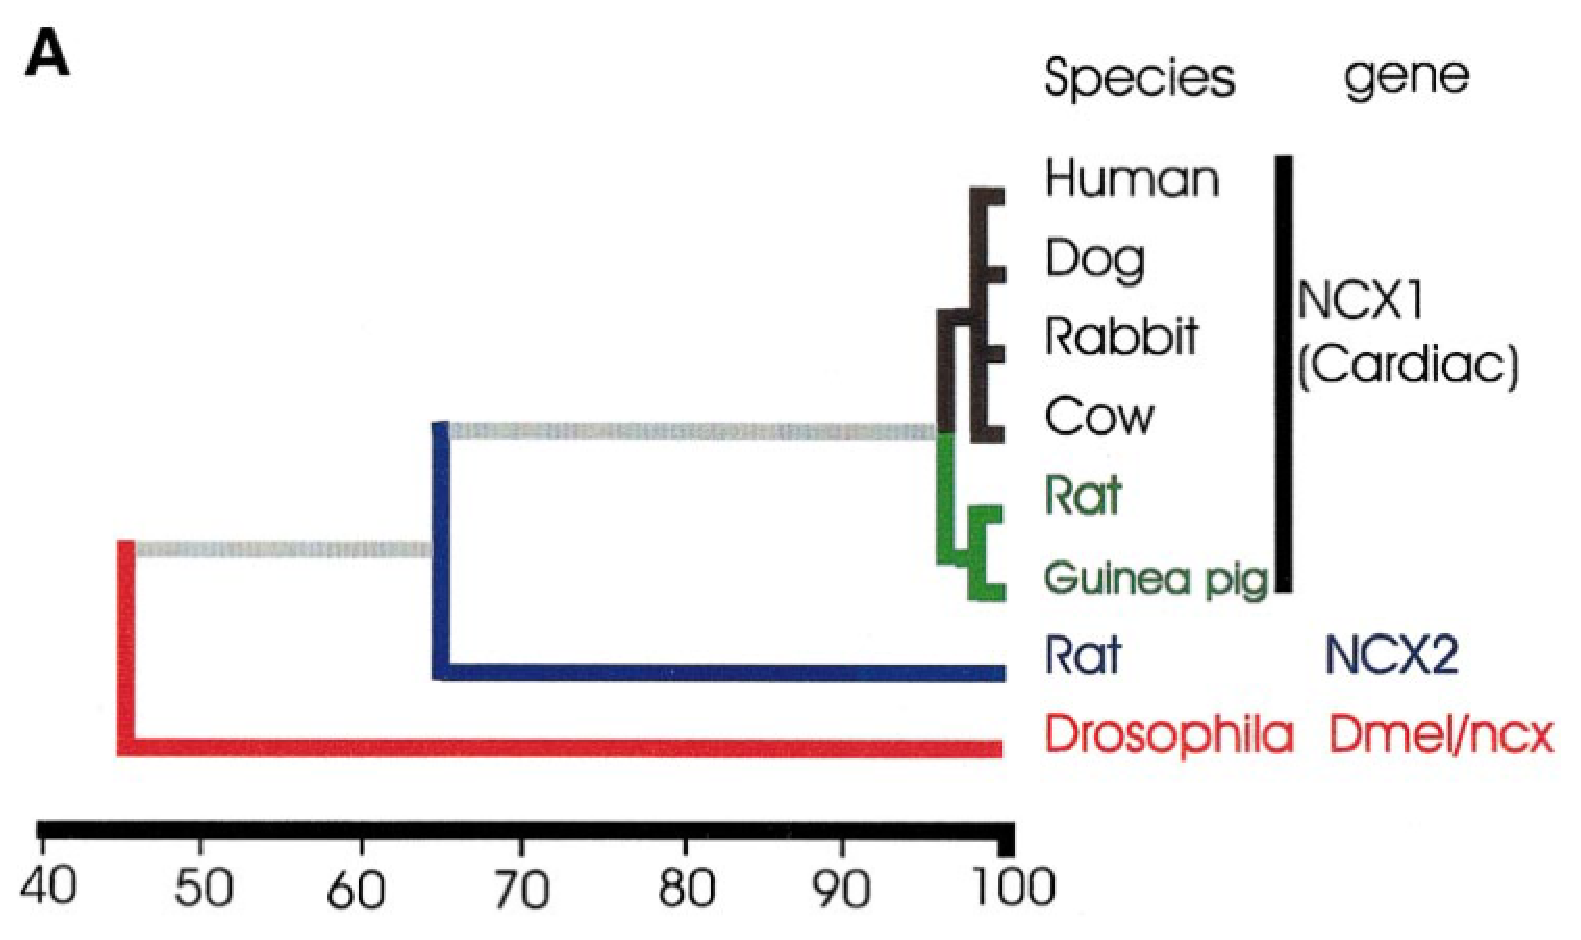
\includegraphics[height=5cm,
    angle=0]{./images/NCX_aa.eps}}
\caption{Percentage of amino acid identity}
\label{fig:NCX_aa}
\end{figure}

NCX1-3 share about 70\% amino acid identity.
\begin{itemize}
  \item NCX1 are found dominantly in heart, brain, and to a lesser extent in
  other tissues
  
  \item NCX2 and NCX3 are expressed in a few limited tissues, such as brain, and
  their molecular properties and functions remain unclear.
  
\end{itemize}


%\subsection{structural conformations}

Its 3D structure has just known since 1994~\citep{}.
\begin{itemize}
  \item  Cardiac NCX1 has molecular mass of 110 kDa. During biosynthesis, its N-terminal
is cleaved off to yield a mature protein.

On SDS-PAGE, under a reducing condition, the mature NCX1 protein often appears
as 2 bands with molecular mass of 120 kDa and 70 kDa (and a faint 140 kDa and
160 kDa band); in which the 70kDa is considered as the proteolytic fragment of
the 120-kDa protein.

Approximately half of the NCX1 protein constitutes a transmembrane domain (TMs),
whereas the remaining half (about 550 amino acids) forms a large domain exposed
on the cytoplasm. The mature NCX1 protein comprises 9 TMs and a large
hydrophilic loop between TMs 5 and 6, with N- and C-termini located on the
external and internal sides, respectively, Fig.\ref{fig:NCX-structure}, and a
large hydropholic loops between TMs 5 and 6.
Two internal repeat sequences of about 40 amino acids called $\alpha-1$ and
$\alpha-2$ repeats are conserved in all members of NCX family as well as in
related cation exchangers suggesting the functional importance of these
segments. 

\begin{figure}[hbt]
  \centerline{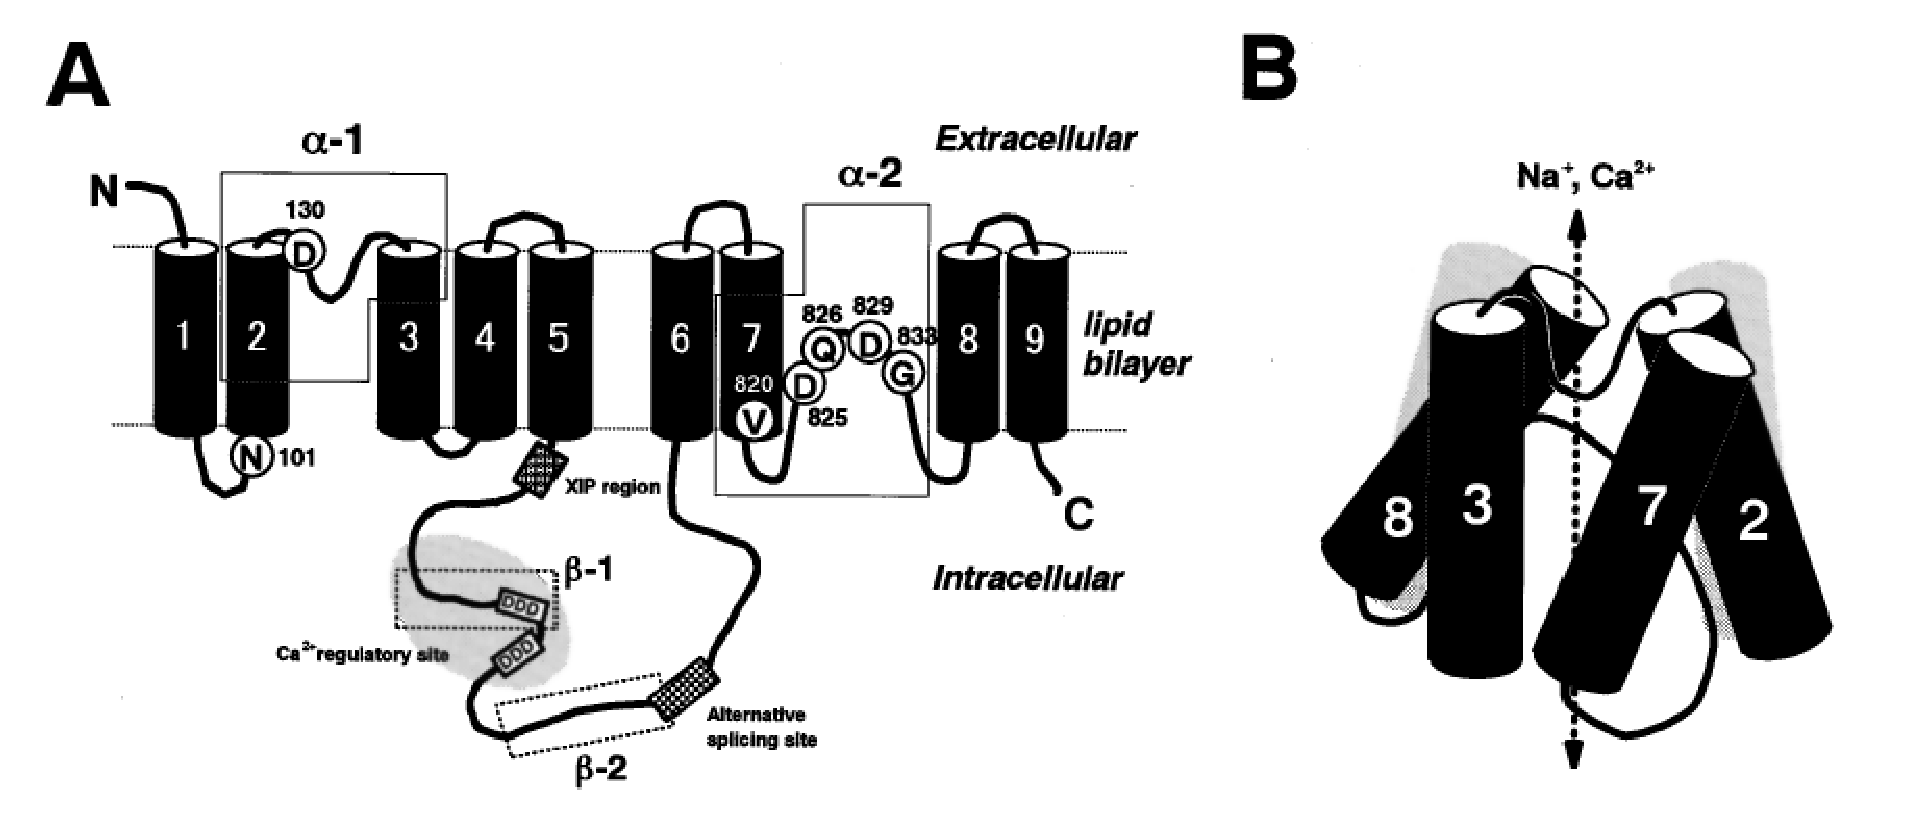
\includegraphics[height=3cm,
    angle=0]{./images/NCX-structure.eps}}
\caption{NCX structure: (A) 9 TM helices are indicated by cylinders, N-terminal
is extracellular and C-terminal is intracellular; (B) Model of helix packing of
TMs 2,3,7 and 8 \citep{shigekawa2001}}
\label{fig:NCX-structure}
\end{figure}

Interactions of NCX1 with the transport substrate
(extracellular Ca2+), inhibitors (Ni2+ and KB-R7943), and an
activator (Li+) are significantly influenced by the mutation of
residues in the a repeat loops. Mutations:
\begin{enumerate}
  \item mutation of conserved glycines (Gly138 and Gly837) alters the slope of
  the current-voltage relationship of NCX1. 
  
  \item mutation of Thr103 at the cytoplasmic portion of TM2 increases the
  apparent affinity of NCX1 for the substrate intracellular Na+ and also seems
  to produce Li+ transport capacity, suggesting alteration in the ionic
  selectivity of the exchanger.
  
  \item number of amino acid residues in the $\alpha$ repeats
whose mutations significantly alter the transport properties of cardiac NCX1:
\begin{itemize}
  \item  mutations of 3 conserved aspartic acids (Asp130, Asp825, and Asp829)
result in up to 6-fold reduction in the apparent affinity for the substrate,
extracellular Ca2+.

  \item mutations of other residues in the $\alpha$ repeat loop regions (Asn125,
  Thr127, and Val820) render the exchanger up to 8-fold less sensitive to
  inhibition by external Ni2+ - a competitive inhibitor for the transport
  substrate, extracellular Ca2+.
  
  \item Val820, Gln826, and Gly833 in the $\alpha$-2 repeat loop, whose
mutations alter the apparent affinity for the inhibitor 
2-[2-[4-(4-nitrobenzyloxy)phenyl]ethyl]isothiourea methanesulfonate (KB-R7943)

Mutation at Gly833 renders NCX1 almost insensitive to inhibition by KB-R7943.
Simultaneous mutations of Val820 and Gln826 alter the extent of stimulation of
NCX activity by external Li+.

\end{itemize}

  \item the putative TMs 4 and 5 contain regions of similarity to the
  Na+/K+-ATPase and SR Ca2+-ATPase, and mutation of Glu199 or Thr203 in
TM5 results in the loss of NCX activity

Glu199 of NCX1 corresponds to Glu309 of SR Ca2+-ATPase.

  \item deletion of a large portion of the central cytoplasmic loop
  ($\Delta$240-679) making NCX1 is not regulated by intracellular Ca2+,
  intracellular Na+ or PKC.

The large cytoplasmic loop is most likely to be involved in the regulation of
NCX activity.

The two $\approx$ 70-amino acid internal repeat motifs, designated
the $\beta$ repeats in the large cytoplasmic loop, are conserved in NCX family.
The functions of these $\beta$ repeats are not clear.

  \item XIP region (a 20 amino-acid segment at N-terminal end of the cytoplasmic
  loop above and near the membrane-lipid interface): is in both basic and
  hydrophobic residues, as in the calmodulin-binding domain.
  
This region, to which calmodulin does not seem to bind strongly, is considered
to play a pivotal role in the regulation of NCX activity.

  \item intracellular Ca2+-dependent regulation:
  
At C-terminal to the XIP region, there is a region of about 135 amino acids
(amino acids 371 to 508) containing 2 conserved clusters of acidic amino acids.
This 135-amino acid region, when expressed as a fusion protein and assayed
directly, binds Ca2+ with high affinity. NCX1 mutants carrying mutations
within the acidic clusters exhibit markedly lowered affinity for regulatory
intracellular Ca2+, suggesting that Ca2+ binding to this region is responsible
for intracellular Ca2+-dependent regulation of NCX activity.

\end{enumerate}
Until 2001, however, little is known about the detailed
structure of the NCX1 molecule, in particular, the ion-binding
sites and the shape and dimensions of the ion transport
pathway, the requirement of the oligomeric protein structure
for the function, and changes in the conformation of the
exchanger associated with ion transport.


  \item NCX2

\end{itemize}



\subsection{-- NCKX1-2}



\subsection{NCX distribution}
\label{sec:NCX-distribution}
%\subsection{Distribution}

\begin{enumerate}
  \item In Smooth muscle - Sect.\ref{sec:NCX-distribution-smooth-muscle}
  \item In cardiac cells - Sect.\ref{sec:NCX-distribution-cardiac-cells}
  \item in brain - Sect.\ref{sec:NCX-brain}:
  astrocyte (Sect.\ref{sec:NCX-glial-cell}); neurons (Sect.\ref{sec:NCX-distribution-neurons})
\end{enumerate}


\subsection{-- Smooth muscle}
\label{sec:NCX-distribution-smooth-muscle}

In both freshly isolated or cultured smooth muscle cells, NCX are
found at regions of plasma membrane that are closely apposed to the
junctional SR/ER. This is in contrast to uniform distribution of
PMCA. 

\subsection{-- Cardiac cells}
\label{sec:NCX-distribution-cardiac-cells}

In the cardiac muscle, only NCX1 isoform is found \citep{shigekawa2001,
minelli2007}. NCX2 and NCX3 are not expressed in adult rat heart at the protein
level, but an NCX2-specific transcript can be detected faintly by using reverse
transcriptase-polymerase chain reaction.

NCX1 expression reaches a maximum near birth and then decreases postnatally to a
significantly lower level in the adult stages. This is in contrast to SR
Ca2+-ATPase (Sect.\ref{sec:SERCA-distribution}), which is increasingly expressed
postnatally.

With NCX1, there are controversial results.~\citep{frank1992} postulated that
NCX is found predominantly in T-tubules; while ~\citep{kieval1992} reported NCX
is uniformly distributed. ~\citep{chen1995}, using rabbit hearts, shown that NCX
appear in all of the ``external'' membrane, although it may be more prevalent in
T-tubule. During the development of the cell, NCX present on the surface
membrane first, and later appear along the Z-line of heart cells as the T-tubule
develop. Recent results suggested NCX1 is distributed 60\% in the T-tubules and
40\% in the sarcolemma.

The kinetics of NCX in cardiac myocyte have been extensively investigated
(Reeves \& Sutko, 1983; Miura \& Kimura, 1989; Crespo, Grantham \& Cannell, 1990;
Khananshvili, 1991; Matsuoka \& Hilgemann, 1992; Niggli \& Lederer, 1993).

\subsection{-- Brain}
\label{sec:NCX-brain}

NCX1-3 are abundantly expressed in several brain areas, often with overlapping
distribution. To date (year 2007), detailed anatomical survey of NCX isoforms
expression in various elements of CNS in situ is yet to be accomplished.



\textcolor{red}{NCX  are present at high concentration in presynaptic
terminals}.

\subsection{++++ Glial cells}
\label{sec:NCX-glial-cell}

NCX1-3 immunoreactivity (ir) was detected in astrocytes (perisynaptic glial
processes).

\subsection{++++ Neurons}
\label{sec:NCX-distribution-neurons}


NCX1-3 were widely expressed in both brain areas:
\begin{itemize}
  \item NCX1 : exclusively found in neuropilar puncta 
  
  \item NCX2, NCX3: found in neuropilar puncta, and also neuronal somata and
  dendrites
\end{itemize}

The properties of NCX in isolated nerve terminals (synaptosomes) were studied in
\begin{enumerate}
  \item rat brain: Fontana, Blaustein (1995) - they suggested NCX accounts about
  1/3 of the total $\Ca$ influx in synaptosomes under resting conditions. 
  

  \item 
\end{enumerate}

Neocortex and Hippocampus:
\begin{itemize}

  \item  In both neocortex and hippocampus, all NCX isoforms were prominently
  expressed in dendrites and dendritic spines contacted by asymmetric axon
  terminals, whereas they were poorly expressed in presynaptic boutons.
\end{itemize}


A very abundant of NCX is expressed at high concentrations in
presynaptic nerve terminal. So, it may play a role in modulation
$\Ca$-dependent neurotransmitter release, as well as $\Ca$
homeostasis.


... (see \citep{blaustein1999})


Species???

On membrane or t-tubules ???


% \subsection{Roles }
% \label{sec:roles-}
% 
% In ECC???

\subsection{Mechanisms of exchange}
\label{sec:mechanisms-Ca2+-exchange-via-NCX}

There are 3 different, controversial and unresolved hypothesis:
\begin{enumerate}
\item {\bf consecutive} or {\bf ping-pong} mechanism: the exchanger
  can bind only one species of transported ion at a time. An example
  is $\Ca$ bind to the cytoplasmic side, no $\Na$ or $\Ca$ can bind
  to, until $\Ca$ is unbound or transported to the ECF and
  dissociate~\citep{khananshvili1995}.

\item simultaneous binding mechanism, where both  $\Na$ and $\Ca$ can
  bind to the exchange at the same time. An example is 3$\Na$ bind to
  the cytoplasmic side and 1$\Ca$ bind to the ECF. When all sites are
  occupied, the exchange undergo a conformation change the transport
  3$\Na$ to the outside and bring 1$\Ca$ to the inside.
\item {\bf sequential}: a variant of the consecutive model, with the
  order of binding/release are different. For example: when $\Ca$ bind
  to inside and transported to the external side, but it needs $\Na$
  bound to before $\Ca$ can be dissociate~\citep{milanick1991}. So,
  the main difference to the consecutive mechanism is that there's at
  least one conformation that both $\Ca$ and $\Na$ bind to the
  exchange. 
\end{enumerate}


\begin{figure}[hbt]
  \centerline{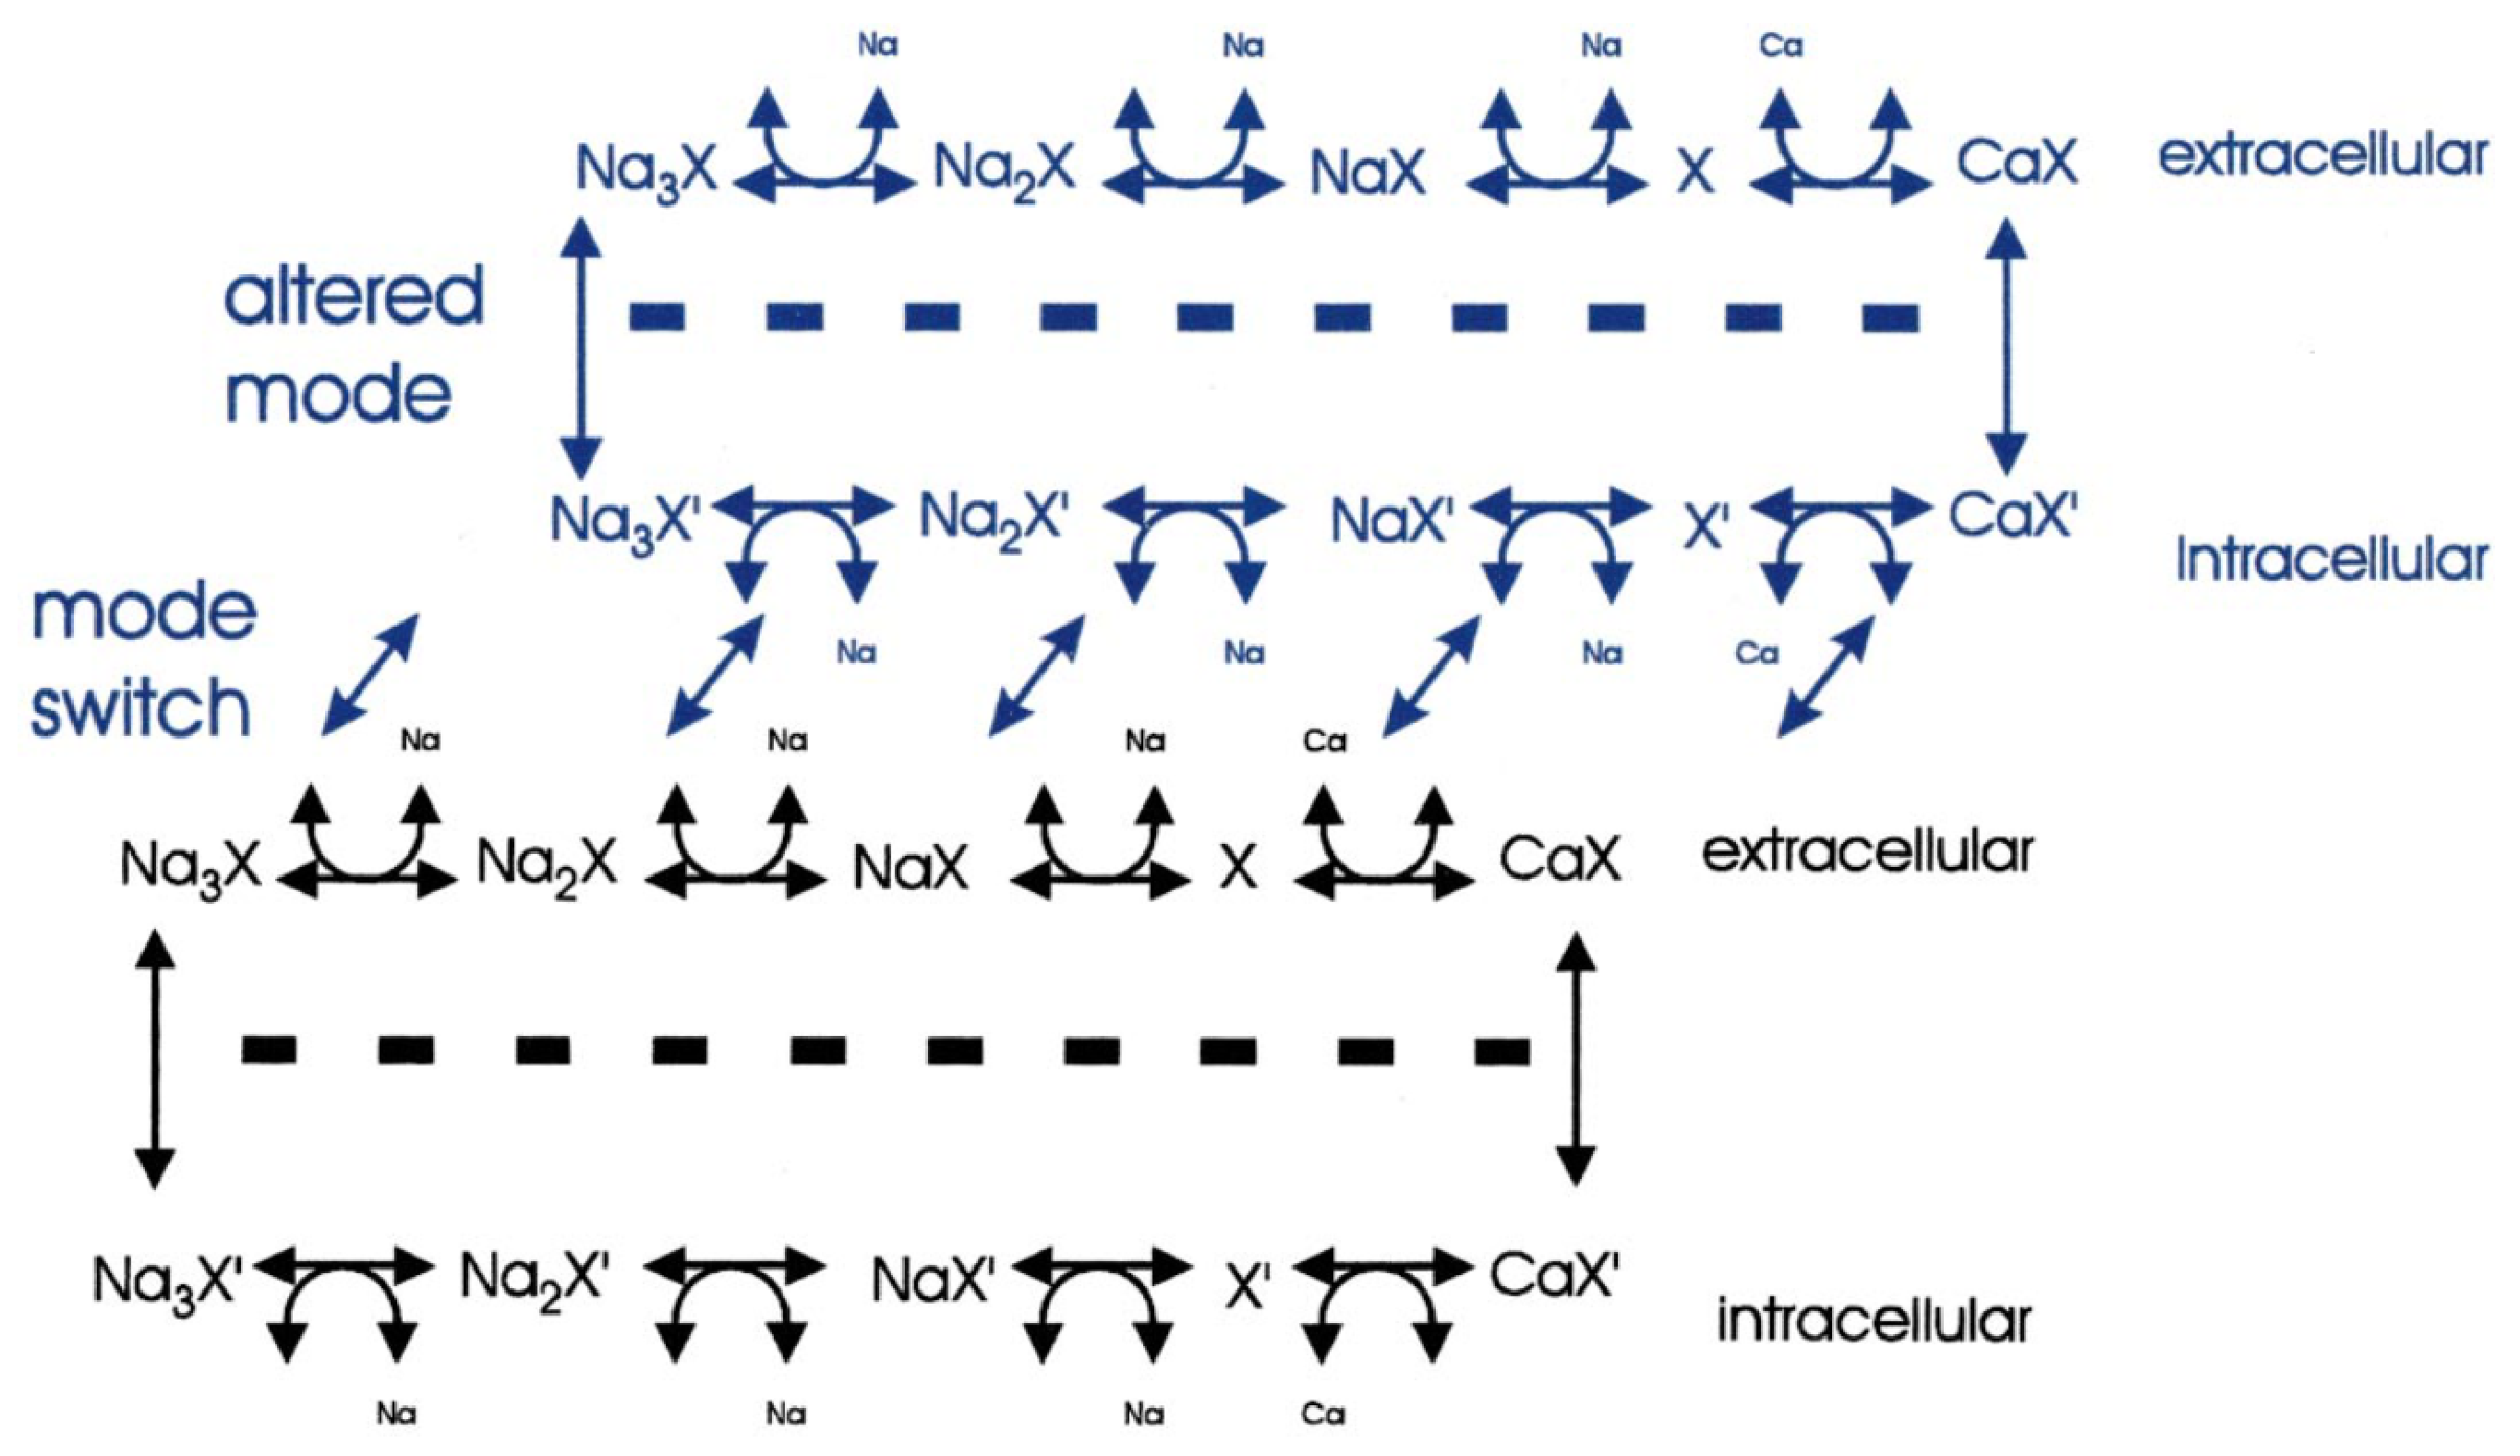
\includegraphics[height=5cm,
    angle=0]{./images/NCX_Blaustein.eps}}
\caption{Schematic diagram of an mode-switching NCX model}
\label{fig:NCX_Blaustein}
\end{figure}



\section{Na/Ca exchanger}
\label{sec:naca-exchange}

Na/Ca exchanger (NCX) is the \ce{Ca^2+} transporter in the sarcolemma
of the heart that is largely responsible for extruding the \ce{Ca^2+}
that enters via $I_{Ca}$. NCX stoichiometry is generally accepted
3Na:1Ca which means that the extrusion of 1Ca is coupled to the inward
of 3Na \citep{egger2000pbn,kang2004mtm}. Remember that the direction of
the electric current is opposite to the direction of electron
(negative charges).  Hence, the corresponding ionic current is
$I_{NCX}$ is inward when extruding \ce{Ca^2+}. Mnemonically, in this
case, $I_{NCX}$ is of the same direction as the influx of \ce{Na+}.

$I_{NCX}$ is reversible and its direction and amplitudes are
controlled by \ce{Na+} and \ce{Ca^2+} on both sides of the biomembrane
as well as by membrane potential $E_m$.  At rest, \ce{Ca^2+} extrusion
is favored thermodynamically as $E_m$ is negative to $E_{NCX} =
3E_{Na} - E_{Ca}$, even the low [\ce{Ca^2+}]$_i$ limits the rate of
\ce{Ca^2+} extrusion. During AP upstroke, $E_m$ passes $E_{NCX}$; so
\ce{Ca^2+} influx and $I_{NCX}$ outward are favored. However, this
period is very short-lived because the very high local [\ce{Ca^2+}]
(owing to SR Ca release and Ca influx) drives $E_{NCX}$ back larger
than $E_m$, hence $I_{NCX}$ becomes inward and extrudes \ce{Ca^2+}
again. As a result, $I_{NCX}$ is an inward current throughout most of
the AP under normal conditions.

{\bf NOTE:} In heart failure (HF), in which SR Ca release is low,
[\ce{Na+}] is elevated, and AP duration (APD) is long, the situation
can be reversed such that $I_{NCX}$ is outward throughout most of the
AP~\citep{weber2003drs}.

In addition to the above-described regulation of NCX flux by
thermodynamics of ion gradients and the kinetic constraints related to
substrate (Na and Ca) concentration, there is also
{\it allosteric regulation} mediated by local [\ce{Ca^2+}]$_i$ and
[\ce{Na+}]$_i$ \citep{philipson2000sce}. Particularly, at high local
[\ce{Na+}]$_i$ (i.e. beyond physical range $>20\mu$M), $I_{NCX}$ is
inactivated.
\textcolor{red}{However, it is unclear that under which physiological
  conditions, can Na-dependent inactivation occurs to a significant
  extent}.
Nevertheless, this dependency can be helpful as it can prevent or
limit consequent cellular \ce{Ca^2+} overload. Also, allosteric
activation occurs at low [\ce{Ca^2+}]$_i$. It makes sense that a
\ce{Ca^2+} efflux would be turned off to prevent [Ca]$_i$ from falling
to low and \ce{Ca^2+} efflux should be more active when [Ca]$_i$ is
high.

Beside allosteric inactivation, we also have allosteric activation of
NCX which results from high [\ce{Ca^2+}]$_i$ in myocytes ($K_{0.5}
\approx 100$nM).
\textcolor{red}{However, the actual \ce{Ca^2+} dependent regulation is
  not well understood}.

There are some other dependency and some remains highly controversial
\citep{bers2008cca}.  $I_{NCX}$ can significantly influence AP shapes,
and the late plateau phase of most atrial and rodent ventricular APs
can be almost entirely due to inward $I_{NCX}$. However, it is
sometimes inappropriately considered as a minor current during AP.
\textcolor{red}{The actual physiological importance of this
  Ca-dependent regulation is not well understood}


\section{\texorpdfstring{\ce{H+}-ATPase}{4. Proton-ATPase}}
\label{sec:H-ATPase}

The plasma membrane potential in most non-animal eukaryotes (e.g. fungi and
plants) is maintained by proton-ATPases, which exports one $\H$ for every one
ATP hydrolysed. Here, there is no counter ion or proton transported in the
opposite direction. This is not the main topics of the chapter though. 

The resting membrane potentials in fungi and plants can be -150mV to -300mV
\citep{morth2011}.
Proton ($\H$) ATPase (type IIIA): to generate membrane potential (which
  is proton potential or potential defined by proton gradient) in fungal and
  plant cells \citep{slayman1970}, and maintain intracellular pH $\sim 6.6$ vs.
  extracellular pH $\sim 3.5$, giving membrane potential -180mV.
  
\section{5. H/K-ATPase and K/H-ATPase}
\label{sec:H/K-ATPase}
\label{sec:K/H-ATPase}

\begin{itemize}
  \item H/K-ATPase (type IIC) (abbreviation: HKA): 2H/2K exchange ($\Na$ can
  substitute for $\H$, and other monovalents for $\K$). They are found in gastric parietal cells (to
  acidifies the stomach) and renal collecting ducts. This is drug target, e.g.
  inhibited by omeprazole - a potent anti-ulcer drug that prevents the
  excess production ofstomach acid.
  
  \item K/H-ATPase (type IIC): they are found in distal colon, thus giving it
  the name {\it distal colon ATPase}, with 2K/2H exchange; kidney, uterus and
  endothelial cells
\end{itemize}

\section{Na/H-exchanger (NhaA)}
\label{sec:NhaA}
\label{sec:Na-H-exchanger}

The 3D structure of the Na+/H+ exchanger NhaA from {\it Escherichia coli} has
been solved, which reveals that it has a highly asymmetric molecular
organization comprising 12 TMs and exists as dimer.

\section{Pumps on neurons}

Ion pumps are distributed over the entire cell membrane but
are particularly clustered in areas with high ion fluxes, such as
the soma, the nodes of Ranvier, and at pre- and postsynaptic
sites.

%%% Local Variables: 
%%% mode: latex
%%% TeX-master: "mainfile"
%%% End: 
